\chapter{Methodology}
%\subsubsection{Overview}
%The methodology section will cover the preliminary work required to get calpy, fast entropy and the classification system working, and the design choices behind the experiments carried out. \\
%
%"This section will cover what was done to in order to classify data correctly. This includes:" \\
%

\subsubsection{Chapter Contents Overview}
This chapter contains: 

\begin{enumerate}
\item Data Collection - What data was used, why and where it was taken from 
\item Code Base - The design of the code and what was required to run
\item Preliminary Testing - Testing the calpy software
\item Pause Analysis - Design choices of pause analysis experiments 
\item Symbolisation - Designing the initial symbol set tests
%\item Entropy - Entropy Parameters
\end{enumerate}

%DATA COLLECTION
\newpage
\section{Data Collection}
\subsection{Talkbank}
%The Talkbank audio files chosen mainly to get pauses are studied, understood and in their application to useful classification. 
The Talkbank files were used as the initial audio files and to gauge the effectiveness of the calpy system for classification. They provided lots of data and were chosen for a number of reasons, including:
%This means looking for audio files with the most natural conversations that would match its intended end result. Initially, Talkbank was used as it provides conversations in a much more relaxed and natural environment, much closer to the actual efforts and application the entropy classifier is hoping to be used for. The files are also provided free for public, welcoming reproducibility of the experiments. Initially, the Talkbank files were the only ones that were going to be relied on. However, higher quality files were introduced later.  \\
%
%
%\paragraph{Reason for databank choice:} 
%Talkbank provided:
\begin{itemize}
	\item A large, open source collection of conversations (1000's of audio files),
	\item Natural conversations (better representation of how pauses are used naturally),
	\item Easy to download,
	\item A diverse range of conversation group types including,
		\begin{itemize}
			\item Age,
			\item Language,
			\item Sex,
			\item Conversation topics,
			\item Multiple conversation types (callHome and callFriend),
			\item Multiple dialects (southern vs northern english),
		\end{itemize}
	\item Recordings were done in stereo (allowing for pause code visualisation),
	\item Long conversations (30 minutes usually).
%	\item natural conversations (beneficial later on when building models for how natural pause use can be expected to be distributed)
%	\item Previously used in the PauseCode paper (making this established and vetted for?).
\end{itemize}

With this variety in conversation types it makes it easier to selectively isolate certain groups and gauge the effectiveness of classification in a more controlled way. It also allows for the removal of anything that might bias results of a certain group (for example how age might influence the effect language has on pause use). 

\paragraph{Talkbank URL:} The Talkbank audio files were taken from \mathit{media.talkbank.com}. Specifically the url's: 

\begin{itemize} \\
	\item https://media.talkbank.org/ca/CallFriend/eng-n/0wav/ 
	\item https://media.talkbank.org/ca/CallFriend/eng-s/0wav/ 
	\item https://media.talkbank.org/ca/CallHome/eng/0wav/ 
	\item https://media.talkbank.org/ca/CallHome/jpn/0wav/ 
\end{itemize}

The meaning behind the subdirectories above were:
\begin{description} 
\item[ca:] Conversation Adult (Conversations only involving Adults)
\item[eng-s:] english southern (Southern dialect of North American English)
\item[eng-n:] english northern (Northern dialect of North American English)
\end{description}

%Potential downside, audio is trash, could lead to contaminated results

\subsection{ABC and JJJ Podcasts}
With the ubiquity of podcasts in recent years and the often high quality recording and production that go into them, podcasts were used after the Talkbank files. While high quality podcasts and interviews allow for cleaner and more reliable results these are usually stilted conversations where flow is controlled to suit the medium of the presentation (conversation caters to the audience), which means talking can become slower, more drawn out, less fluid and less natural and thus may deliver less applicable models for how conversational modelling should occur naturally. However, this was fine for the purposes of this thesis to determine the initial information theoretic properties of pauses and their suitability as a speech classifier.  


%In order to balance out the differences in format between the two podcasts (i.e. to get the same number and sex of hosts) the JJJ Lunch podcast was also proposed to be added into the data set. However, based on the research collected from other tests and the paper [x] it wasn't deemed necessary. Also to balance out the audio length time more JJJ files were used (since the ABC podcasts were roughly 3-4 times longer on average than the JJJ podcasts). \\


\paragraph{ABC Podcast Information:} The ABC podcast files were taken from the program 'Conversations' with hosts Richard Fidler and Sarah Kanowski. \\
Taken from the url https://www.abc.net.au/radio/programs/conversations/episodes/.

\paragraph{JJJ Podcast Information:} The JJJ podcast files were taken from the program 'Mornings' with Linda Marigliano. \\
Taken from the url https://www.abc.net.au/triplej/programs/mornings/. 

\paragraph{Reason for databank choice:} ABC radio and JJJ both provided:

%\footnotesize{
\begin{itemize}
	\item Free and easy to download audio files (aiding in reproducibility),
	\item Easy to handle audio format (mp3),
	\item Wide range of data sources (News, Podcasts, Radio, etc \ldots),
	\item A wide range of interview types across,
	\begin{itemize}
		\item Age,
		\item Nationality,
		\item Topic (comedy, informative, pop culture, news, personal interest, etc...),
	\end{itemize}
	\item High quality audio files,
	\item Ideal recording conditions,
	\item High number of podcasts available,
	\item Long lengths (10-20 minutes usually),
	\item Consistent hosts (allows for better testing of the influence one host has on the conversation).
\end{itemize}

The specific JJJ and ABC podcasts were used to aid in easily categorising by age by finding podcasts on the relative extremes of age (young vs middle aged+elderly). The JJJ Mornings program hosted a lot of interviews with a young interviewer (one female host in her 20's) and interviewees, while the ABC Conversations podcast provided many conversations with middle aged interviewers (one female host and one male host both in their 50's) and elderly interviewees. 
%}

\subsection{File Organisation and Location} 
The folder structure was created to best preserve the original database structure such that finding the file again could be done simply and no files would be incorrectly attributed to another group. All files can be found in the Calpy source code in:

\paragraph{Talkbank\\}
\indent ./data/dialogue/conversations/media.talkbank.org/ca/CallFriend/eng-n/0wav/ \\
\indent ./data/dialogue/conversations/media.talkbank.org/ca/CallFriend/eng-s/0wav/ \\
\indent ./data/dialogue/conversations/media.talkbank.org/ca/CallFriend/jpn/0wav/
\indent ./data/dialogue/conversations/media.talkbank.org/ca/CallHome/eng/0wav/
\indent ./data/dialogue/conversations/media.talkbank.org/ca/CallHome/jpn/0wav/

\paragraph{ABC\\}
./data/dialogue/interview/abc/radio/programs/conversations/

\paragraph{JJJ\\} 
./data/dialogue/interview/abc/jjj/programs/mornings/

%\subsection{Comparison}
%Although neither approaches are perfect, both will be used to gather as much data as possible. Further tests could be done on podcasts that aren't presented so much in an interview settings but rather a conversation between participants to get more natural use of pauses. This wasn't carried out for this thesis paper. This method of using podcasts could also be done for other languages as many podcasts exists in many languages throughout the world. 
%%Currently the only language tests done were on the Talkbank files between English and Japanese. 
%The ABC and JJJ podcasts provide a good insight into the statistics of pauses in a much higher detail than Talkbank as well as providing general information about pause use for classification purposes by determining the general power of the pause algorithms and entropy classifier being used.\\


\subsection{Automated Collection}
Bash scripts were written to pull audio files from Talkbank, create subdirectories and sort files instead of doing these tasks manually. Using wget allowed for automatic downloading of the repository. An example wget command is:

\begin{verbatim}
wget -r -l1 -A.wav https://media.talkbank.org/ca/CallFriend/eng-n/0wav/
\end{verbatim}

Another script was used to automatically create and sort files into organised directory folders. This looped over all the files and created directories for the original audio recording and the resampled recording that Calpy required. This was done many times to download many different directories of content but only for Talkbank as the number of files was in the hundreds. \\

For the ABC files, a download button was provided on the page, however the JJJ files did not present one. The JJJ audio pages had to be inspected using the 'inspect' tool provided by most browsers to find the link used by the html/js code to load and play the mp3. Following that link led straight to a downloadable version of the audio file.

\subsection{Audacity Format Translation} Although most of the actions could be automated through scripts, all the resampling had to be done manually and individually. Downloading from the data bank provided either mp3 or wav. WAV was inline with Calpy's implementation so that was used. However, the audio needed to be reformatted into higher resolution in order for calpy to do proper analysis. \\

Files were manually fed to audacity to put into the correct audio format. Often the files taken from the databanks couldn't be understood either because of sampling problems or the file format used (e.g. mp3). Audacity served as a reliable translator of media formats and frequencies. Care was taken to preserve as much of the original audio as possible. The Talkbank files were saved as 16000 khz from 8000khz to try increasing the audio clarity (no difference occurred in results). Results of the resolution experiment can be found in the results. The Talkbank files were kept as stereo files. ABC and JJJ were saved as their original format of 48,000khz. The ABC and talkbank files were kept as their original format of mono while JJJ was kept as stereo. Although the JJJ files were stereo they did not split the audio effectively, thus both channels contained all the same audio information. However, the Talkbank files were properly recorded in stereo. \\

Resolution increased linearly with digitisation time. Although Talkbank files were low in quality (i.e. low digitisation time per file, roughly 1-2 minutes), they were high in number (roughly 350 files in total) requiring lots of time to spend on this process. The ABC radio and JJJ files also took longer (roughly 20 minutes each) due to the high quality of the audio files but were significantly less in number than the Talkbank files. The digitisation process put a threshold on how much data could be processed. Initially only a few ABC radio and JJJ files were digitised. Only the digitisation process requires large time investments, all other procedures in the analysis process are quick. \\






\newpage
\section{Code Base}
This section outlines all the work done to produce the code, the design implementation and what the code can produce. 



\subsection{Set Up}
\subsubsection{Location}
All code can be found in the ./calpy/ directory, the code written for this research can be found in ./calpy/pause/ as well as extra plot code written in ./calpy/plots.

\subsubsection{Libraries Used}
\begin{itemize}
\item pydub.AudioSegment (WAV decoder) 
\item ffmpeg (requirement system install to use AudioSegment)
\item pandas (data handling)
\item numpy (data handling)
\item json (data handling)
\item matplotlib (plots)
\item seaborn (plots)
\item ptitprince (plots)
\item seaborn (plots)
\end{itemize}


\subsubsection{IDE}
Visual Studio Code was used to write everything due to its flexibility, lightweight and ease of use with running terminal commands.

 
\subsection{Design}
\subsubsection{Design goals}
The main goal was to make the code as sturdy, modularised and abstracted from the pause implementation as much as possible. It was also designed to be as readable and easily useable by others as possible. The main goals being:
\begin{itemize}
	\item Usability
	\item Replicability (for results)
	\item Error free (no bugs)
	\item System invariant (should work on windows and unix)
	\item Implementation invariance (i.e. if other prosodic speech elements are incorporated in the future, it should be trivial to incorporate)
\end{itemize}

Calpy already had a number of packages to use (e.g. DSP, plots, rqa, etc..). A pause package was created that sat on top of these functions, this included:
\paragraph{audio\_file\_.py:} All work required to digitise, symbolise, perform entropy and produce plots are done through the AudioFile class
\paragraph{data\_handling.py:} Data manipulation and formatting
\paragraph{dataset\_functions.py:} Collections of audio\_files were processed here
\paragraph{file\_handling.py:} Reading and writing to disk
\paragraph{parameters.py:} All initial input parameters for pause digitisation, symbol models, fast entropy settings and plot settings 
\paragraph{dataset\_folder.py:} Stored arrays of all the directories, files, frequencies and audio augmentations used \\

Modularising the code in this way made it more easily updatable, readable, design invariant and less prone to bugs. In total the pause package is roughly 1200-1300 lines of code. All audio files belong to an audio\_file\_ object that contains all the variables used and allows for meta-analysis on groups of audio\_file\_ objects all at once (e.g. histograms showing the difference in pauses amongst all the pause files). This minimised a lot of redundant work as the code generally had to be run over and over to ensure results were correct. All Audio files can be run by simply calling the directory, files and frequency from pre-defined arrays. An example of the main code can be seen in Figure 5.1: 
\begin{figure}[h]
	\begin{center}
		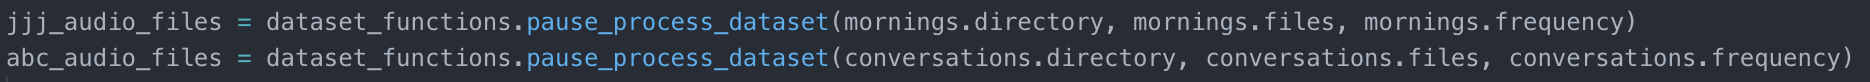
\includegraphics[scale=0.5]{src/main-matter/methodology/code-base/code/main}
		\caption{The code required in main to analyse all JJJ and ABC podcasts. This was designed to be as simple to compute as possible}
		\label{default}
	\end{center}
\end{figure}

These two lines create a collection of audio\_file\_ objects that can be used collectively. An example dataset can be seen in Figure 5.2.\\
\begin{figure}[h]
	\begin{center}
		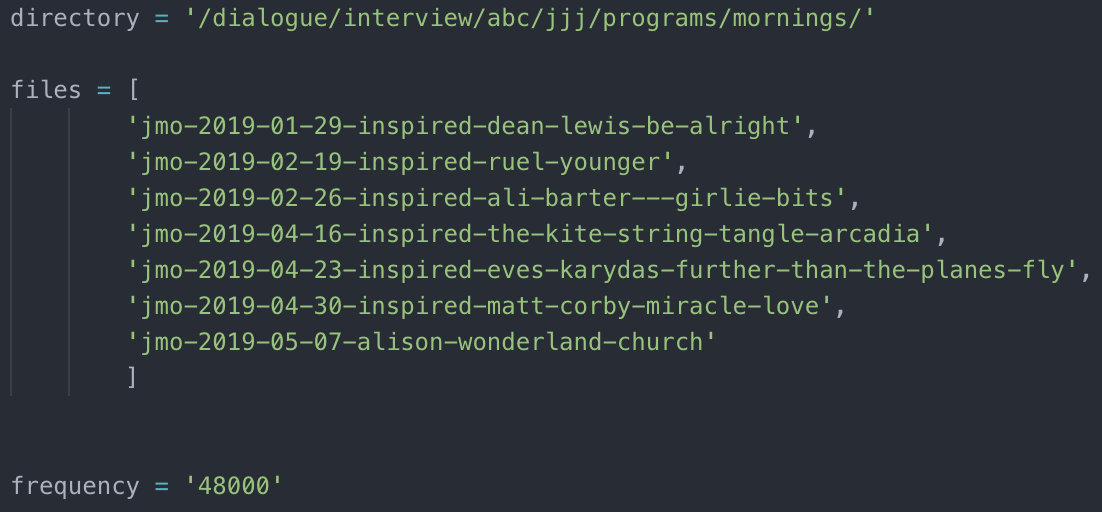
\includegraphics[scale=0.7]{src/main-matter/methodology/code-base/code/dataset}
		\caption{JJJ Mornings Dataset showing a list of files in a specified directory and their corresponding frequency}
		\label{default}
	\end{center}
\end{figure}
Test datasets were also made to ensure calpy is working and for finding bugs. These files are significantly lower in size than the actual files used (which can take 10-20 minutes to digitise). \\

\subsubsection{AudioFile Class}
AudioFile is split into 4 main parts:

\begin{enumerate}
	\item Digitisation
	\item Symbolisation
	\item Entropy
	\item Plots
\end{enumerate}

In brief, an audio file specified in main is turned into an audio\_file\_ object, this object will digitise the audio, symbolise it, produce the entropy profile, plot everything needed and output all variables calculated to file automatically. Each section requires input parameters to customise the output (e.g. min\_silence, bin\_sizes, symbol\_model, etc...). An example of the parameters of a given run can be seen in Figure 5.3. Everything produced from these sections finishes by writing to files and then reading them back. This effectively makes a checkpoint in the code that can be picked up on from later. Examples of the output variables can be seen in Figure 5.4 and 5.10-14. Once audio is digitised every other action can be done almost immediately with the saved digitised binary pause output. 

%Although this is good practice, it was really only worth doing for the digitisation process as this is the most time demanding. 

\begin{figure}[htbp]
	\begin{center}
		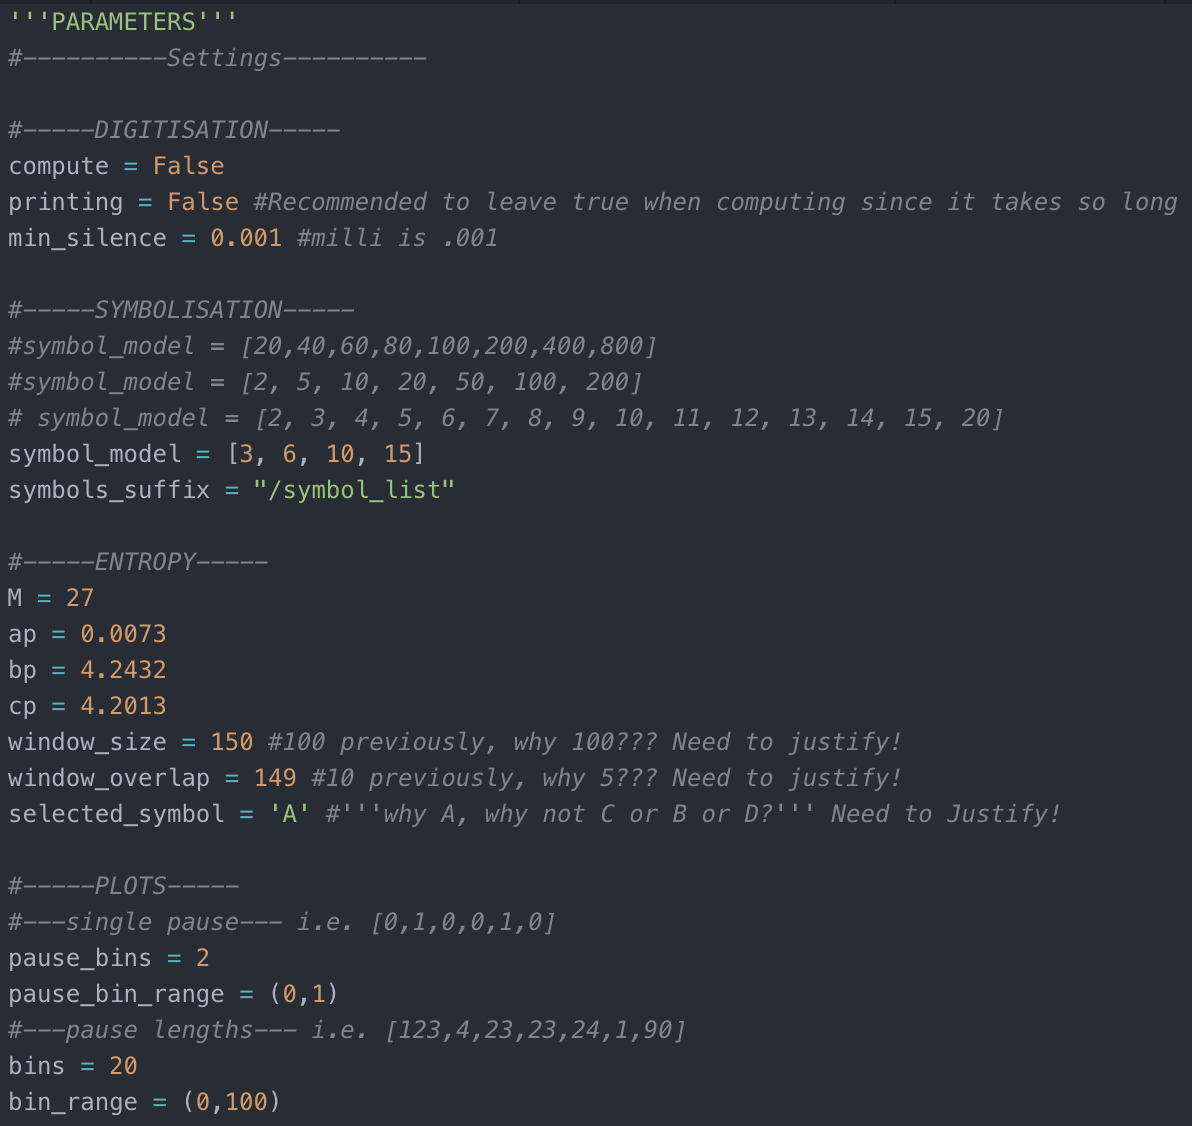
\includegraphics[scale=0.6]{src/main-matter/methodology/code-base/code/parameters}
		\caption{Example Parameter Setting for Calpy. These are required to run the analysis and control such parameters as the entropy window size, symbol model, and whether to recompute the digitised binary pause output}
		\label{default}
	\end{center}
\end{figure}

\subsubsection{Digitisation}
This turned audio files into 1's and 0's. The only parameter present for this section was min\_silence which recorded a pause for a given window of the audio file if a silence was present for as long as the min\_silence time given (e.g. a window of 100ms would be digitised as a pause if there existed a pause of length min\_silence (say 10ms) in that time frame). Min\_silence testing was done at 10ms, 1ms and .1ms and 1ms gave exponentially increasing time costs as the min\_silence value got shorter. \\
%but provided reasonable amounts of data back in terms of binary representations for each. 

Pauses of unbroken length (min of 1ms length used) were looked for and grouped as a single pause, the length of the pause being determined by the number of individual binary pauses that make up that pause. An example of the binary pause output can be seen in Figure 5.4 where a single pause is represented by an unbroken run of 0's, so the first pause from that file would be 2000ms because there is a run of 20 0's at the start of the output. Similarly for utterances where they are represented by 1's. %What about pauses that are unbroken by speech but broken by background sound? Maybe I should say that although we are looking for long pauses, its worth noting that finding long pauses is affected by the quality of the pause isolation. As the pause length goes on its more likely something will break it that incorrectly should not do so. \\

\begin{figure}[htbp]
	\begin{center}
		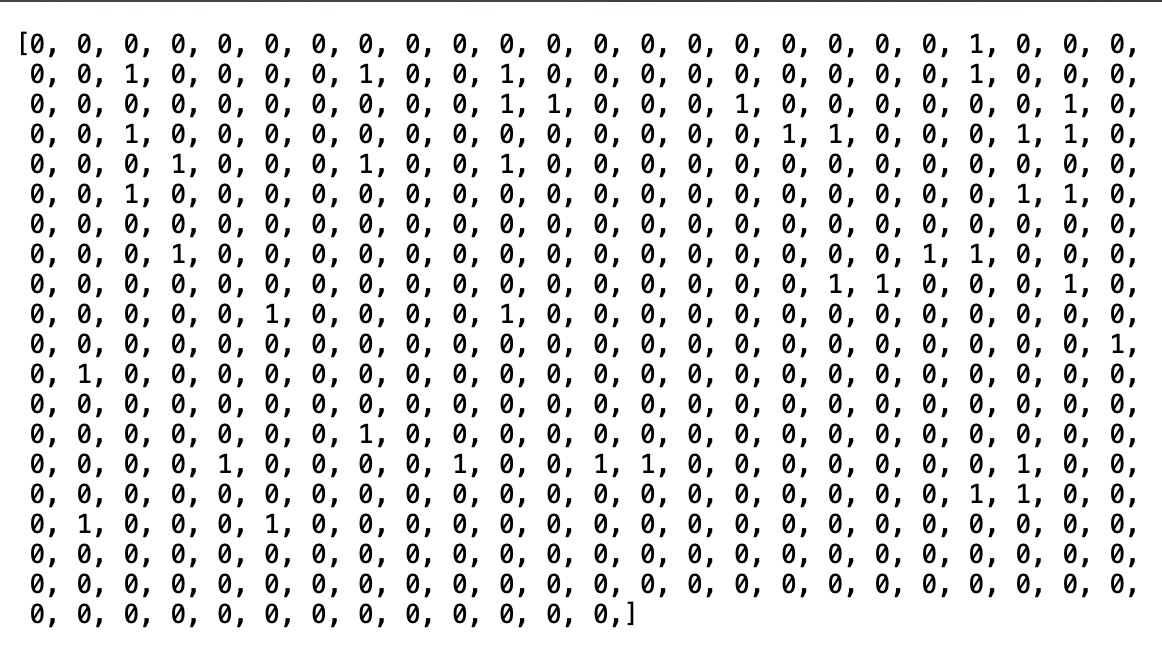
\includegraphics[scale=0.6]{src/main-matter/methodology/code-base/output/binary_pause}
		\caption{Example Binary Pause Output, where a single pause is represented by an unbroken run of 0's. The first pause from this file would be 2000ms because there is a run of 20 0's at the start of the output.}
		\label{default}
	\end{center}
\end{figure}


\subsubsection{Symbolisation}
Symbolisation was written to handle arbitrary symbol models as input without needing to change underlying implementation, meaning any bin size with any number of symbols can be created and modelled immediately (more precisely, the symbol model can be as long as the set of ascii characters). Capital letters are only used for readability purposes but the underlying code is able to use capital and lower case letters, numbers, special characters or any other ascii character as symbols. \\

Theoretically this allows for many types of pauses to be characterised (e.g. joint pause from speaker A to B, or vice versa, or inner pause of speaker A or inner pause of speaker B), however this isn't recommended until much more experiments is done and a much larger database of audio files can be drawn from to increase sample size. The symbolisation then automatically ranks the symbols based on the most frequently occurring to the least. When the symbols are ranked it can often be the case that they will not appear in alphabetic order, showing some pauses to be more frequent that are farther out. As shown in Figure 5.5 where B is the most frequently occurring and A is the least frequently occurring. \\
%Although literature from [paper] posits that there are 64 different types of pauses, it may hinder results to look for each distinct pause as very few samples will be able to be collected for each pause. This was deemed a potential future addition if enough data was found. \\

%While this code can be implemented to look for 64 distinct pauses and symbolise them accordingly, the data might not be sufficient to pull out data like that. 


\begin{figure}[htbp]
	\begin{center}
		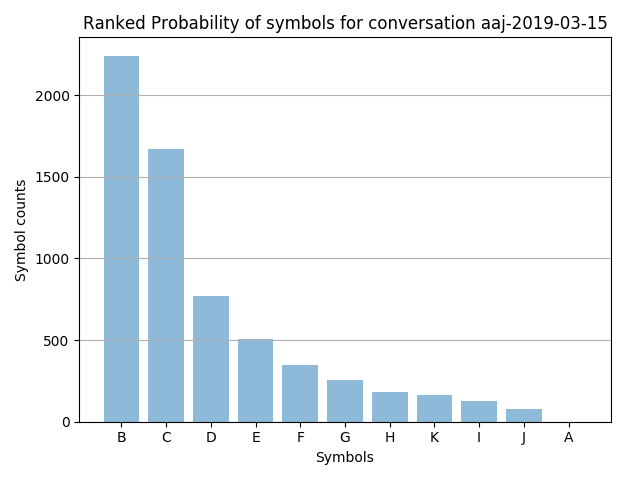
\includegraphics[scale=0.7]{src/main-matter/methodology/code-base/output/ranked_probability}
		\caption{Example Ranked Probability Plot where symbols are ordered by their likelihood of occurrence in the dataset. In this dataset B is the most frequently occurring and A is the least frequently occurring.}
		\label{default}
	\end{center}
\end{figure}

\subsubsection{Entropy} 
The novel Entropy method as outlined in [back] was initially incorporated into Calpy to reduce the computation time needed to produce entropy values. However, initial tests were on files with far greater symbol set sizes than what ended up existing for the audio files, meaning entropy calculations ended up being negligible in terms of time spent. This meant there was no noticeable difference in computation time between classic entropy and the novel entropy in terms of testing. Further tests were done using classic entropy as less parameters were required to be experimented with but the novel entropy was still written for the system. Accuracy change was negligible. 

\subsubsection{Plots}
In order to visualise the data and draw insight various plots were written that included histograms and raincloud plots to visualise pause distributions, utterance vs silence plots to showing the proportion of time spent pausing in an audio file, dual symbol probability ranking plots to show how one symbol set compares to another using the same symbol model, and anomaly plots to show how the entropy values change over time.

\begin{figure}[h!]
	\center
	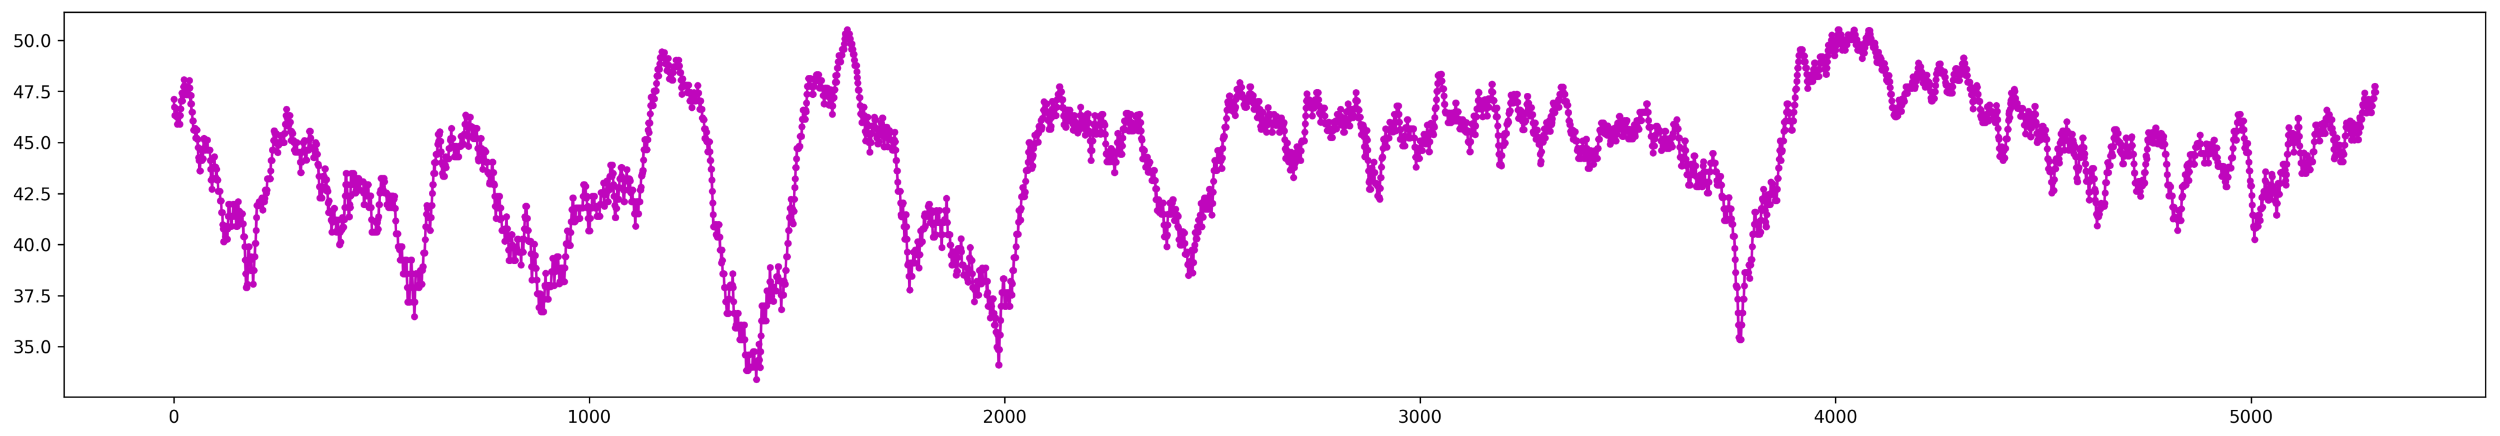
\includegraphics[scale=0.4]{src/main-matter/methodology/code-base/output/output_anomaly}
	\caption{Example Anomaly Plot shows the change in entropy over time for a given audio file. This is used to quickly visualise key properties of the entropy profile.}
	\label{fig:processing}
\end{figure}

\begin{figure}[h!]
	\center
	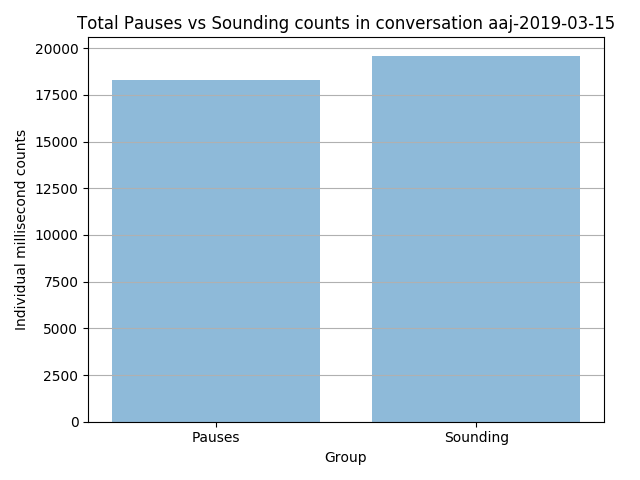
\includegraphics[scale=0.6]{src/main-matter/methodology/code-base/output/binary_pause_bar_chart}
	\caption{Example Sounding Plot shows the proportion of utterance to silence. This example shows an audio file with approximately 55\% of the file being utterances.}
	\label{fig:processing}
\end{figure}

\begin{figure}[h!]
	\center
	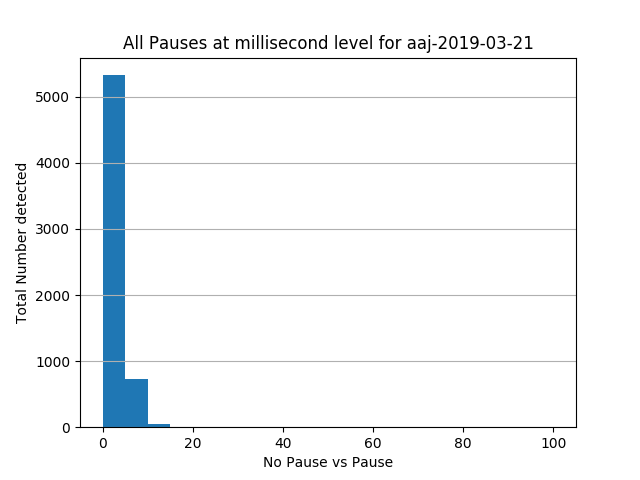
\includegraphics[scale=0.6]{src/main-matter/methodology/code-base/output/pause_histogram}
	\caption{Example Histogram Plot shows the distribution of pause lengths for a given audio file. This example shows a high proportion of audio files clustered around 1000ms.}
	\label{fig:processing}
\end{figure}

%\begin{figure}[h]
%	\center
%	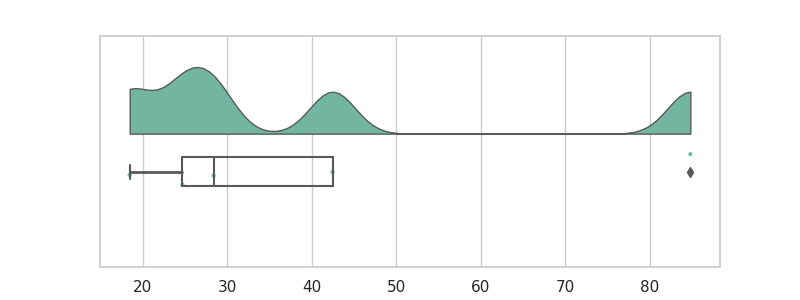
\includegraphics[scale=0.3]{src/main-matter/methodology/code-base/output/raincloud}
%	\caption{Example Anomaly Plot}
%	\label{fig:processing}
%\end{figure}

\begin{figure}[h!]
	\begin{center}
		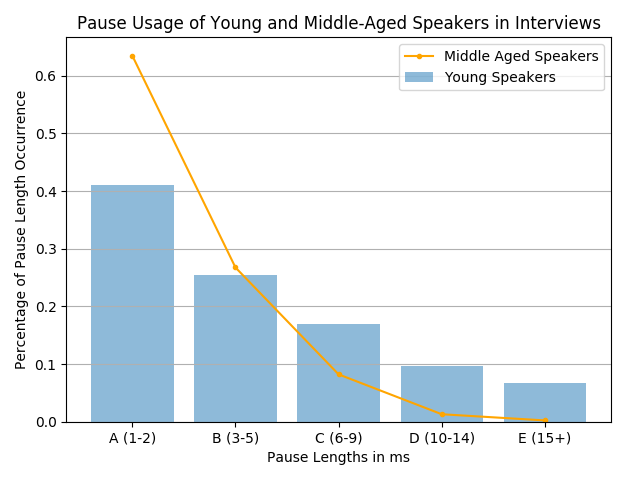
\includegraphics[scale=0.6]{src/main-matter/methodology/code-base/output/dual_ranked_probability}
		\caption{Example Ranked Probability Plot for a symbol model of [3, 6, 10, 15] where two datasets are shown, one in yellow and one in blue. This is useful to see how symbol models perform on audio files of separate groups.}
		\label{default}
	\end{center}
\end{figure}

\subsection{Required Input} All thats required are wav files of correct formatting and their file path. A range of frequencies are usable. Specifically 8000hz, 11025hz, 16000hz, 22050hz, 32000hz, 44100hz, 48000hz, 88200hz, 96000hz were all tested and accepted.

\subsection{Output} Upon completion all relevant output is automatically saved into a file structure dictated by the input folder structure (except now located in the output folder). Example: The file located at: 
\begin{verbatim}
'./data/interview/abc/jjj/programs/mornings/'
\end{verbatim}
would be output to 
\begin{verbatim}
'./output/interview/abc/jjj/programs/mornings/'.
\end{verbatim}

This was done to make file processing easier so only a file directory and a list of names was needed to process everything at once. 
It also allowed for easy reanalysis based upon work that had already been done without having to recompute previous work (which is costly). 
In order to streamline the process of gathering results, all variables generated throughout the procedure were sent to a text file (with some also being used in plots). Example text output files are shown below: \\

\begin{figure}[h!]
	\center
	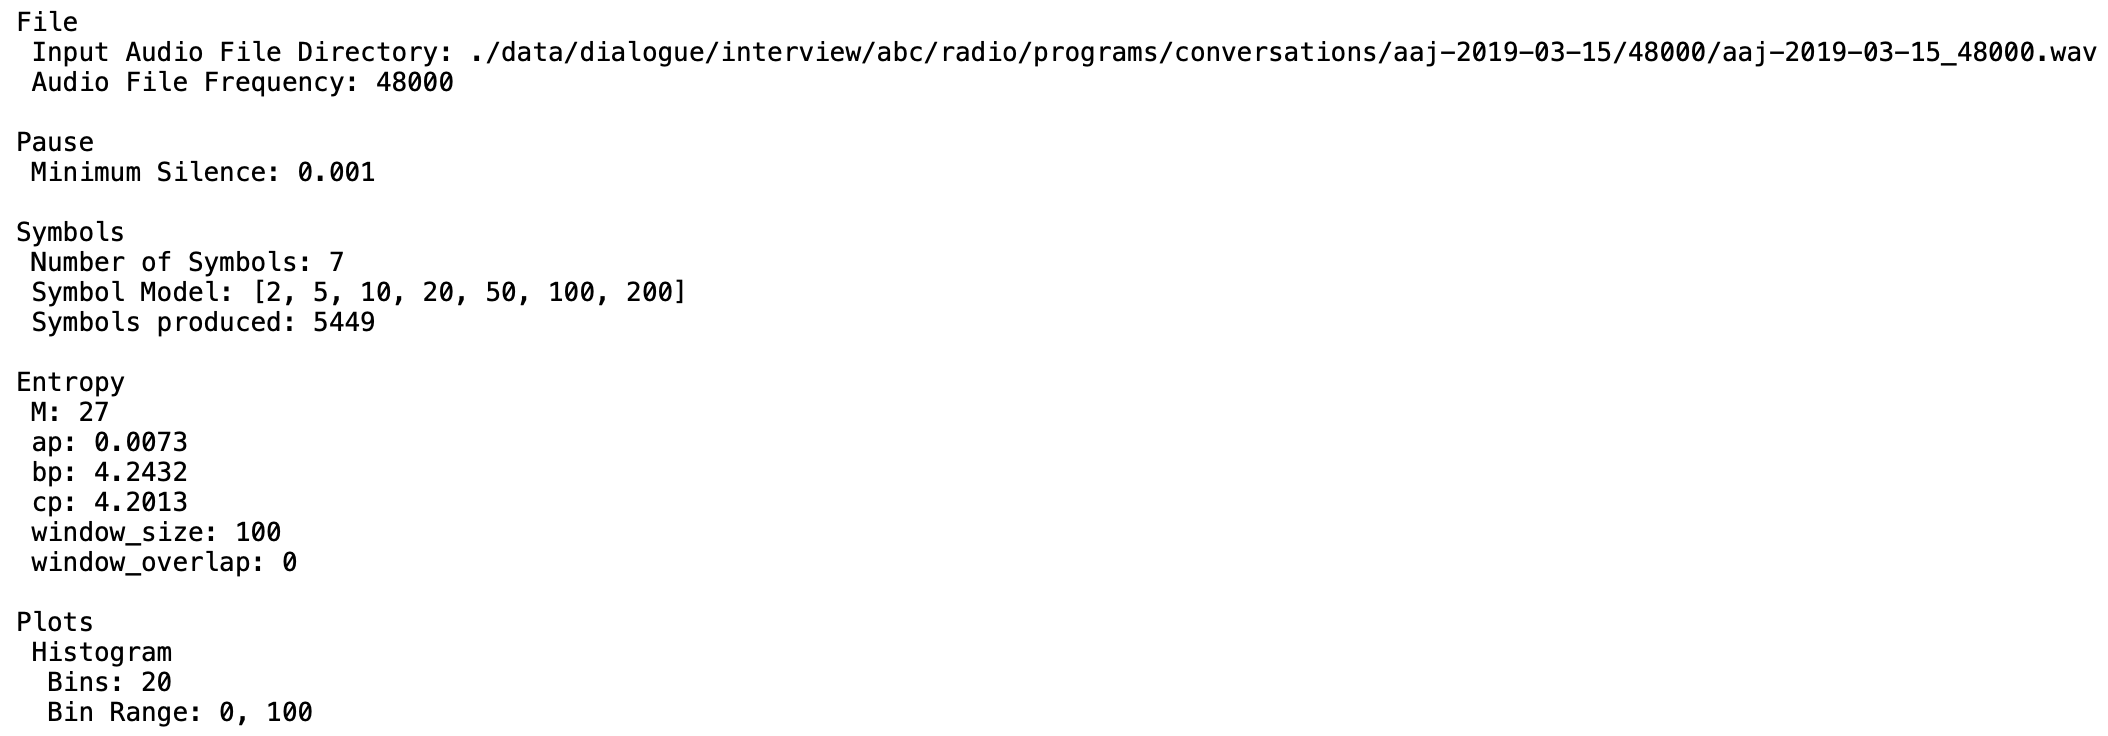
\includegraphics[scale=0.4]{src/main-matter/methodology/code-base/output/input_parameters}
	\caption{Example Code Parameters show what is recorded to disk after every program run. This ensures the correct input parameters can always be referred back to for any test or experiment that was performed.}
	\label{fig:parameters}
\end{figure}

\begin{figure}[h!]
	\center
	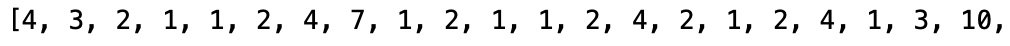
\includegraphics[scale=0.7]{src/main-matter/methodology/code-base/output/pauses}
	\caption{Example Pause Output shows what the pauses look like for an audio file. Each number represents a single pause of that length multiplied by 100ms. These values are derived from the binary pause output.}
	\label{fig:parameters}
\end{figure}

\begin{figure}[h!]
	\center
	
\includegraphics[scale=0.5]{src/main-matter/methodology/code-base/output/output_symbols}
	\caption{Example Output Symbols show what is required to perform entropy calculations. The symbol file will usually span 1000's of symbols.}
	\label{fig:processing}
\end{figure}

\begin{figure}[h!]
	\center
	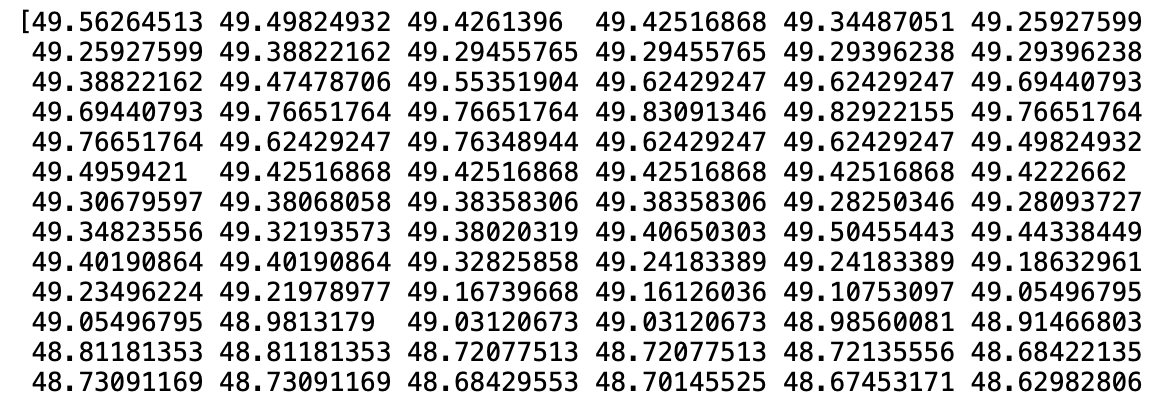
\includegraphics[scale=0.7]{src/main-matter/methodology/code-base/output/output_entropy}
	\caption{Example Output Entropy Profile shows what the entropy profile looks like. Generally the values for entropy are much lower, but specific values aren't important, its the relative change that matters.}
	\label{fig:processing}
\end{figure}

\begin{figure}[h!]
	\center
	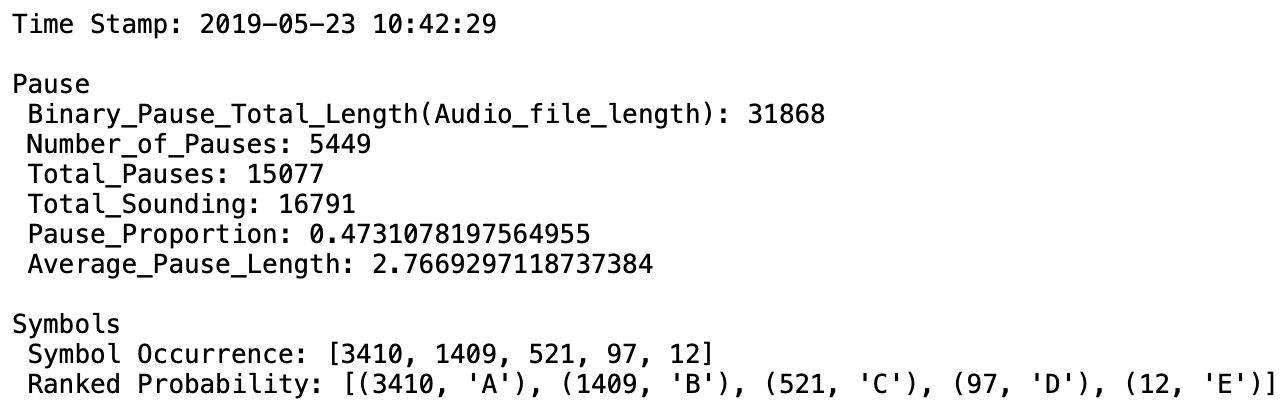
\includegraphics[scale=0.6]{src/main-matter/methodology/code-base/output/output_data}
	\caption{Example General Output Data shows general properties of the audio file and it's pauses. This is produced for every audio file analysed automatically.}
	\label{fig:processing}
\end{figure}


\newpage



\newpage
\newpage
\section{Preliminary Testing}
\subsection{Reason for Experiment}
Before any analysis of the data was done, work was carried out to ensure Calpy behaved as expected and any bugs or potential problems were fixed or documented early. These experiments were designed to measure the effectiveness of the Calpy software using controlled speech where each pause can be counted visually looking at the waveform and artificially constructed precisely using the Audacity software. Then finally testing the software on sample audio files to see what can be expected from the varied chosen datasets. \\

The significance of these tests show the level online systems can be used before being adversely impacted by quality due to noise or compression. In order to build a functioning and useful online system, knowing the limits and strengths of the audio quality can be a major factor in subsequent build requirements. If files require high quality then bandwidth must be high in order for the system to produce meaningful results. This can also affect the equipment used, if a simple inexpensive microphone is used it may place a high cost on the quality of the results due to the amount of compression and information lost through recording to lower quality. This can also affect the environments this can be used in and the placement of recording devices. \\  

\subsubsection{Goals}
\paragraph{1.} Make sure all pauses that are produced are accounted for (not focussing on length, just presence detection)
\paragraph{2.} Make sure all pauses of arbitrary length X are measured correctly by the digital signal processing module and saved accordingly 
\paragraph{3.} See what the difference in quality is like between the two datasets \\

The first two goals ensures that the software is able to extract all pauses distinctly and correctly (in terms of time) for measurement and making inferences from while the third allows for a quick comparison before moving too far forward with the chosen data sets. \\

\subsection{Audacity Testing Overview} 
Real speech was recorded in a quiet environment to make sure no external 
noise was present that could change the outcome. Waveforms were given initial 
stilted dialogue that progressed into more natural and 
relaxed readings of greater time lengths. Pauses were injected into the speech to see that
 it accurately picks up changes in speech in finer grained, controlled levels. 
Finally high fidelity ABC interviews were digitised and analysed to return a benchmark 
of what can be expected from ideal conditions. \\ 

This could be shown in a pause code plot as well to verify the outcomes visually from the 
audio to the analysed Calpy pause code plot, however not all audio files that are used come
in the proper two channel format which pause code requires to distinguish one voice from another.  \\

%The experiments showed Calpy worked as expected bar one exception, Calpy doesn't signal the last pause in the file, meaning any trailing pauses are ignored. 
Almost all pauses were detected correctly and accurately. 
However, the times of the pauses in between words were measured out exactly and distinctly to make 
sure Calpy could pick up the length of each pause. An example of a synthetic audio file is shown in Figure 5.15. \\

Although more tests could be done in this area to further test Calpy's capabilities and 
where it breaks down in terms of rising and falling of voice (thus where pauses are 
determined), these tests showed that Calpy provided enough accuracy to detect the pauses 
and correctly measure all of them from the sample audio files presented, thus allowing for initial tests to commence. \\

\begin{figure}[htbp]
	\centerline{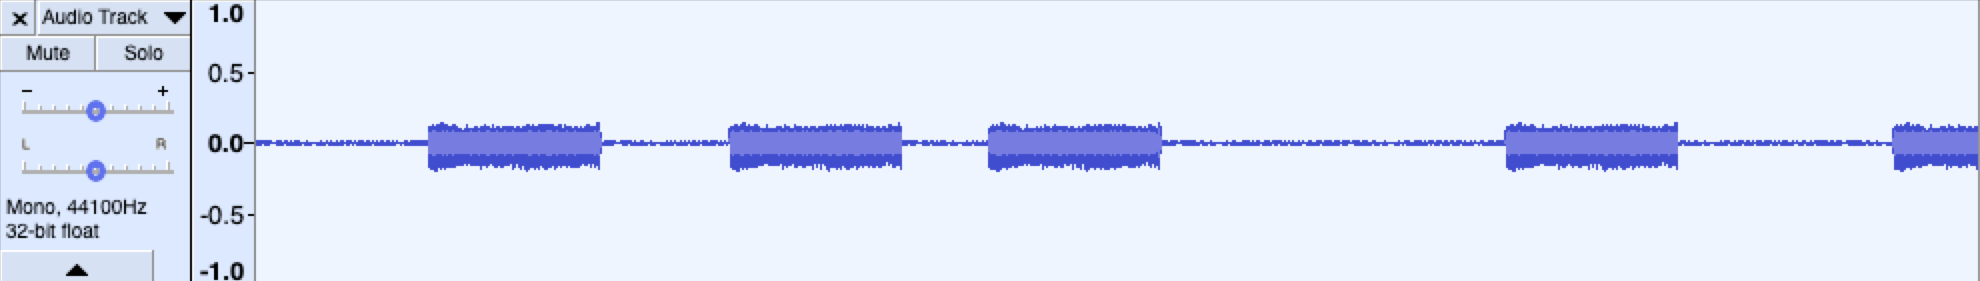
\includegraphics[scale=0.3]{src/main-matter/methodology/preliminary-testing/4170/022}}
	\caption{Example audio file of controlled synthetic utterance and pauses. Each silence is measured out precisely using Audacity}
	\label{flr1}
\end{figure}


\subsection{File format \& frequency}
Mp3 and wav file format were tested, along with the corresponding frequencies from 8000 to 96000 (but only for wav). Testing showed the Calpy software will only accept wav files and not necessarily all wav files either. The original wav audio files had to be converted through audacity first before being digitised, the specific reason was never found. File frequency didn't seem to matter though as Calpy was able to accept anything from 8000+ (this simply increased digitisation time). 
%Knowing how to run Calpy and use wav files correctly took significant troubleshooting. 

\subsubsection{Talkbank}
The Talkbank files could be downloaded in either wav or mp3, however the audio processing library of Calpy does not accept mp3. The wav files were downloaded and transformed through Audacity, taking the mp3 and converting to wav through Audacity to see if this made any difference to results was never tried. The files were available in stereo and could be digitised in either stereo or mono (after transformation through Audacity). 

\subsubsection{Podcasts}
The ABC and JJJ podcasts were available in a high quality wav format. The conditions were in a sound proof room with high quality recording equipment with 2 speakers. These files were really only available in mono, although some files had two channels present when loaded into Audacity the significant overlap of speakers on both channels meant they were effectively mono. Audio files had to be given to Audacity and exported as a wav file with the same file frequency in order for Calpy to accept these files. The right libraries must be imported to handle wav files. Specifically requiring:
\begin{verbatim}
#importing wav
from pydub import AudioSegment #required a brew install ffmpeg
\end{verbatim}

%This was crucial and work could not be done without this installation (this also took significant troubleshooting). 

\subsubsection{Pause Code Plots}
Pause code plots required true stereo so that the file chosen can be split into two channels where each speaker is only in their own channel (i.e. you cant hear the second speaker in the first channel and vice versa). This made the Talkbank files useful for producing the pause code plots. If speaker overlap is present, this will produce a sounding pattern plot that looks like figure 5.16 instead of figure 5.17. \\

Mono audio can't be split into two stereo channels either (channel A with a silent channel B will work, but channel B with a silent channel A will not, not sure why), it must be a stereo split into two mono's. However, significant problems showed up in the pause code when analysed microscopically. The timing of files and their pauses did not match up to the wave form, and some files showed repeated pauses where silence occurred for that speaker (indicating noise present, other speaker was present, or potentially the timing was incorrect for the pause code time stamps). This wasn't investigated further as it wasn't crucial for the investigation (more than likely due to poor audio quality of Talkbank). Examples of incorrect and correct results can be seen below. \\  

\begin{figure}[h!]
	\centerline{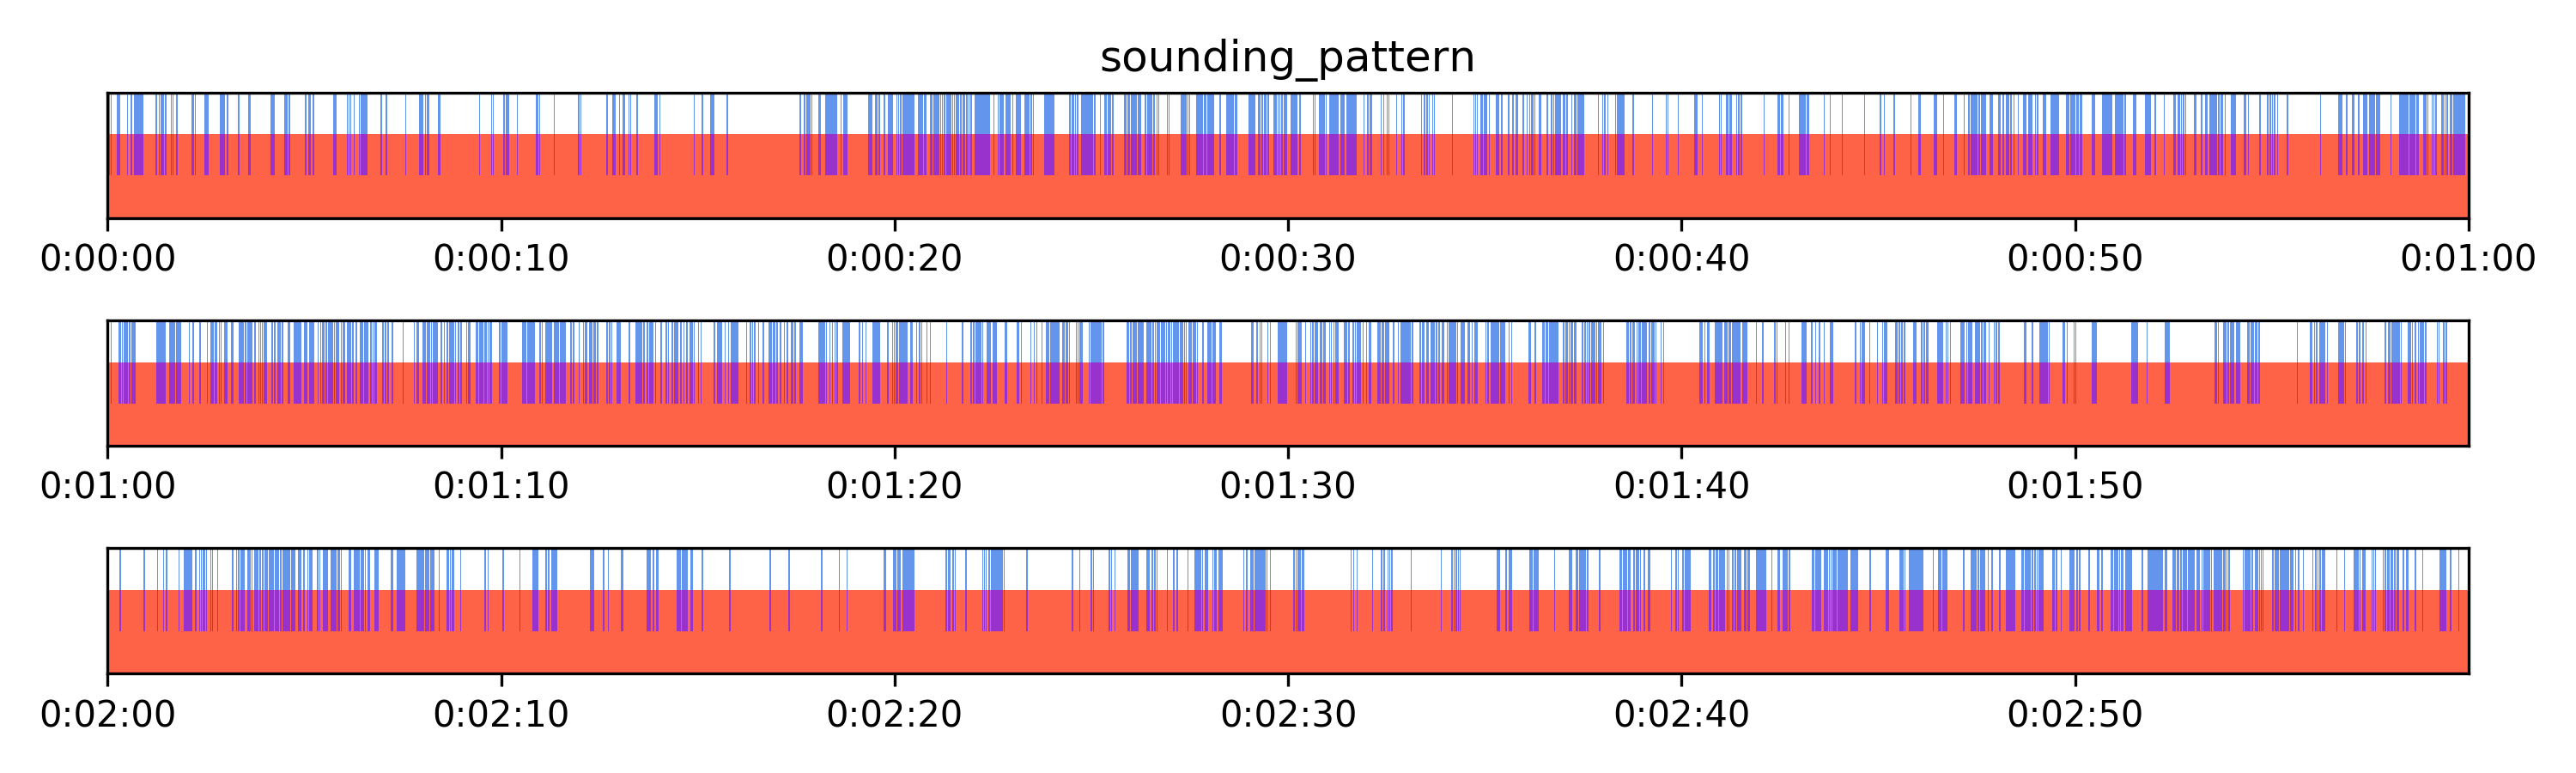
\includegraphics[scale=0.5]{src/main-matter/methodology/preliminary-testing/4170/sounding_pattern_plot_4170_stereo_split}}

	\caption{Entire 4170 - Pause Code Plot - Channel A in blue - Channel B in red. Sounding plot with improper file formatting shows an extended utterance for channel B when no sound exists for that Channel.}
	\label{fig:overlap-sounding}
\end{figure}

\begin{figure}[h!]
	\centerline{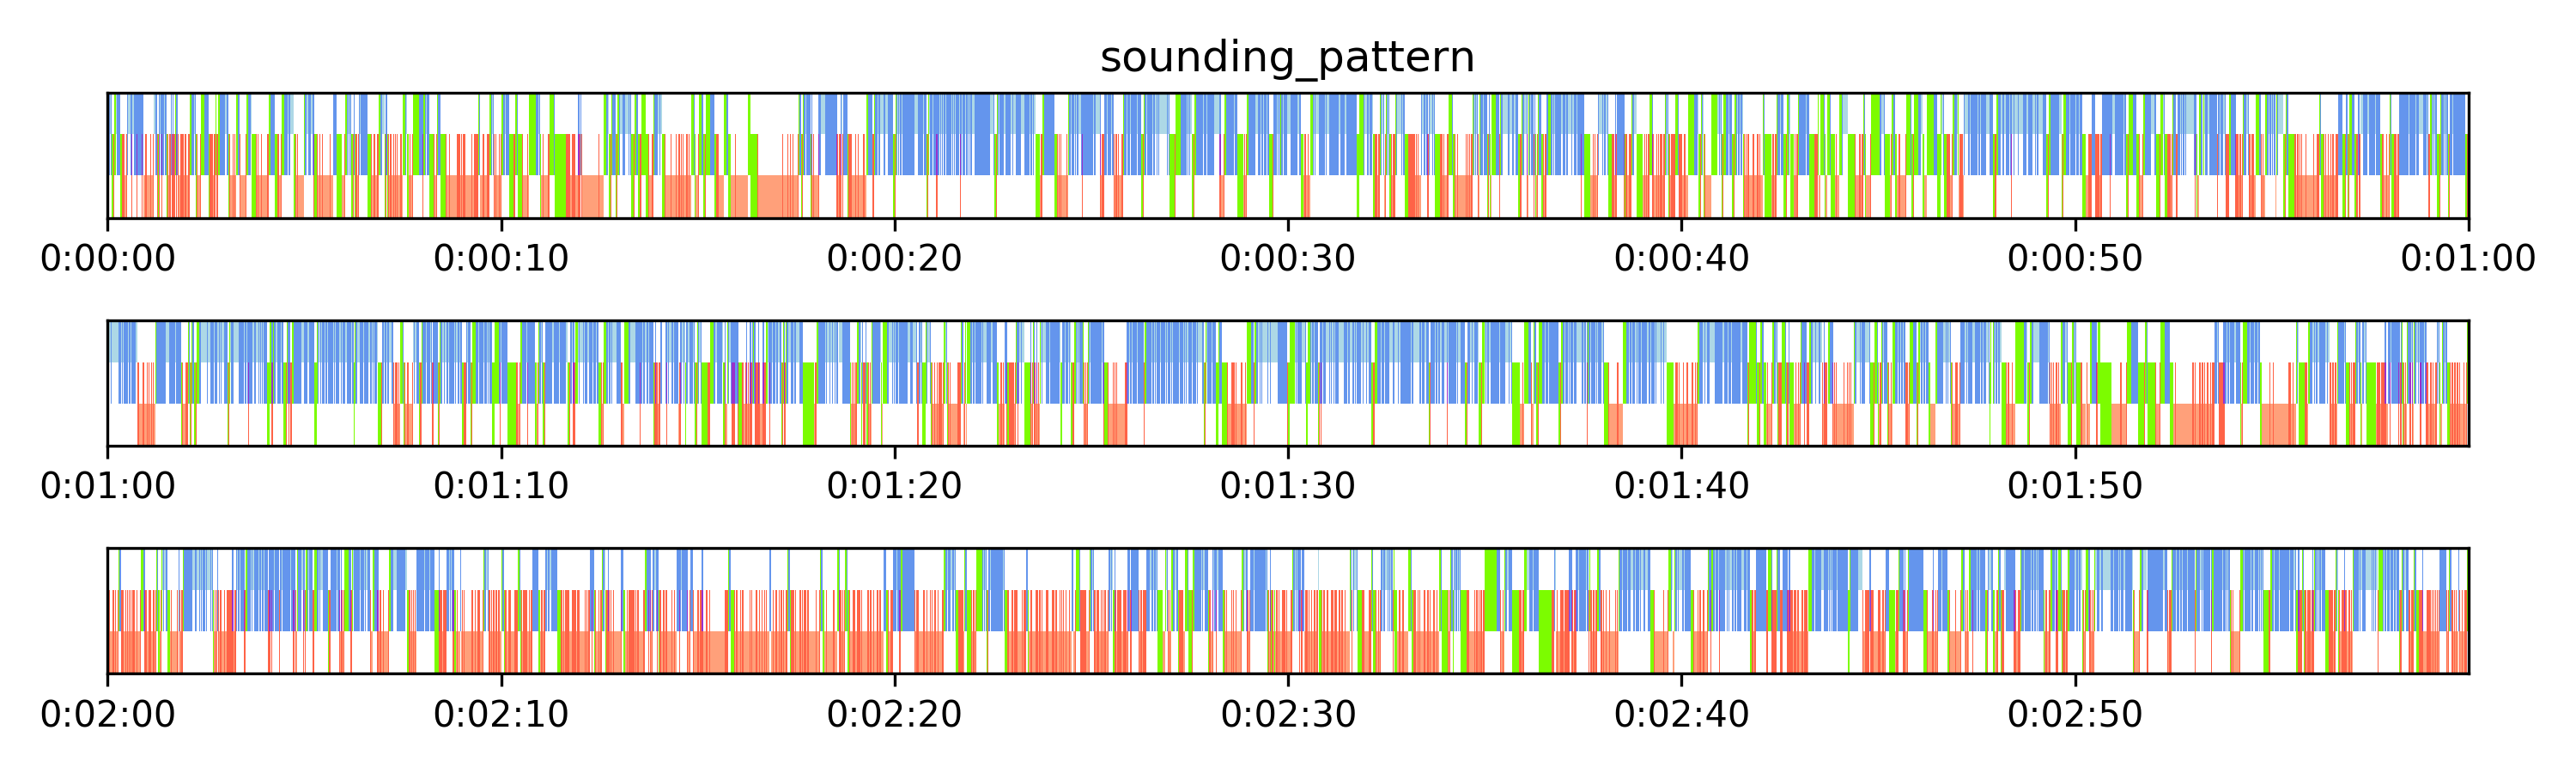
\includegraphics[scale=0.5]{src/main-matter/methodology/preliminary-testing/4170/sounding_pattern_plot_4170_mono_split}}

	\caption{Entire 4170 file - Pause Code Plot - Channel A in blue - Channel B in red. Sounding plot with proper file formatting where both channels are correctly separated and contain different audio tracks.}
	\label{fig:separate-sounding}
\end{figure}

An example of pause code producing incorrect results for two waveforms can be seen in Figures 5.18-21. The wave form shows no audio present for channel B yet utterance can be seen. 

\begin{figure}[h!]
	\centerline{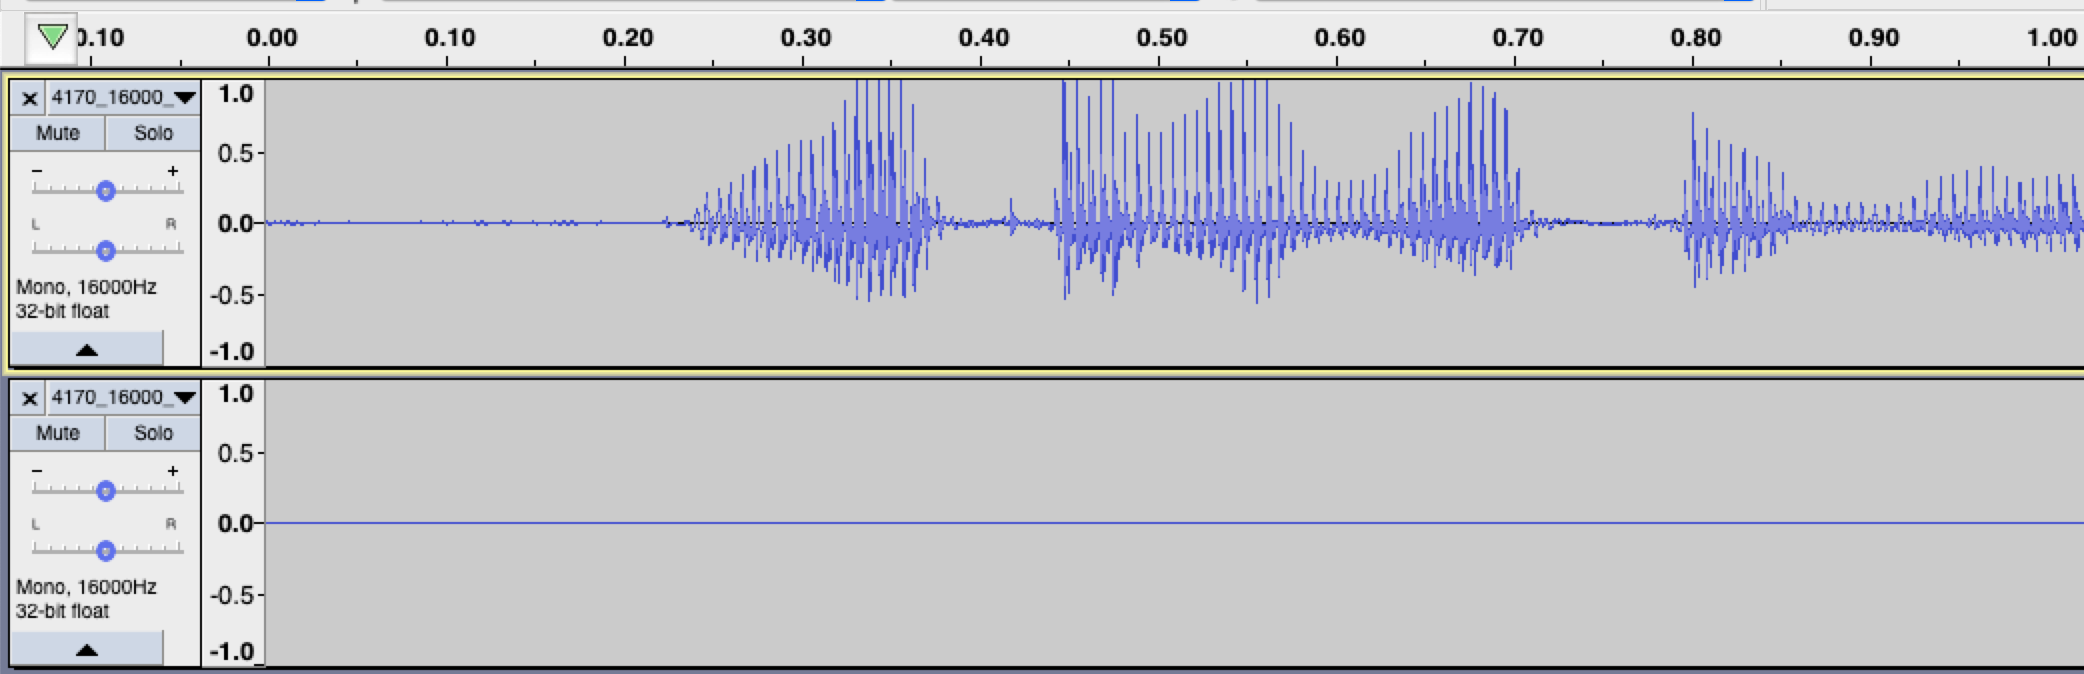
\includegraphics[scale=0.3]{src/main-matter/methodology/preliminary-testing/4170/waveform_4170_1s_chA_top_original}}
	\caption{4170 waveform - The first second of audio - Channel A top, Channel B bottom. Only sound present for Channel A, no sound present for Channel B.}
	\label{fig:upclose_sounding}
\end{figure}
\begin{figure}[h!]
	\centerline{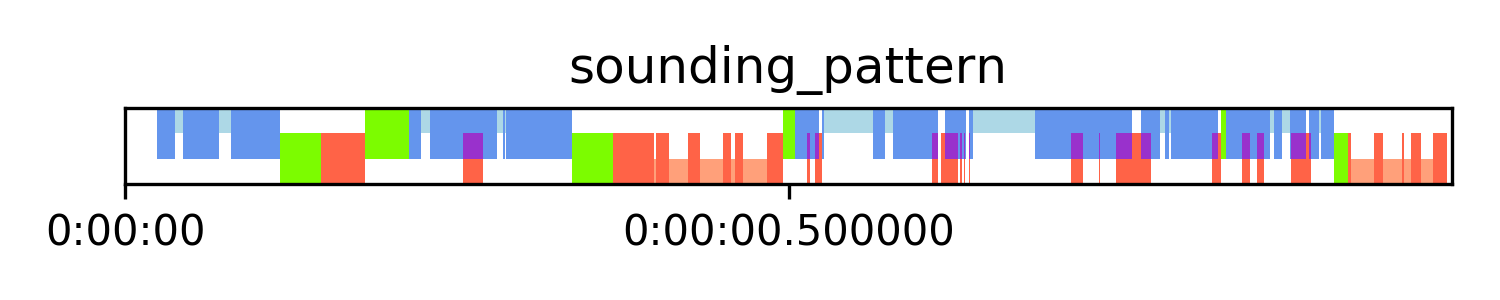
\includegraphics[scale=0.9]{src/main-matter/methodology/preliminary-testing/4170/sounding_pattern_plot_4170_mono_1s_range_short}}
	\caption{4170 Pause Code Plot - The first second of audio - Channel A in blue - Channel B in red. Pause code shows utterances for both channels despite no audio existing for Channel B.}
	\label{fig:upclose_sounding}
\end{figure}

Another example showing pause code producing incorrect results for a five second waveform of the same audio can be seen below. 

\begin{figure}[h!]
	\centerline{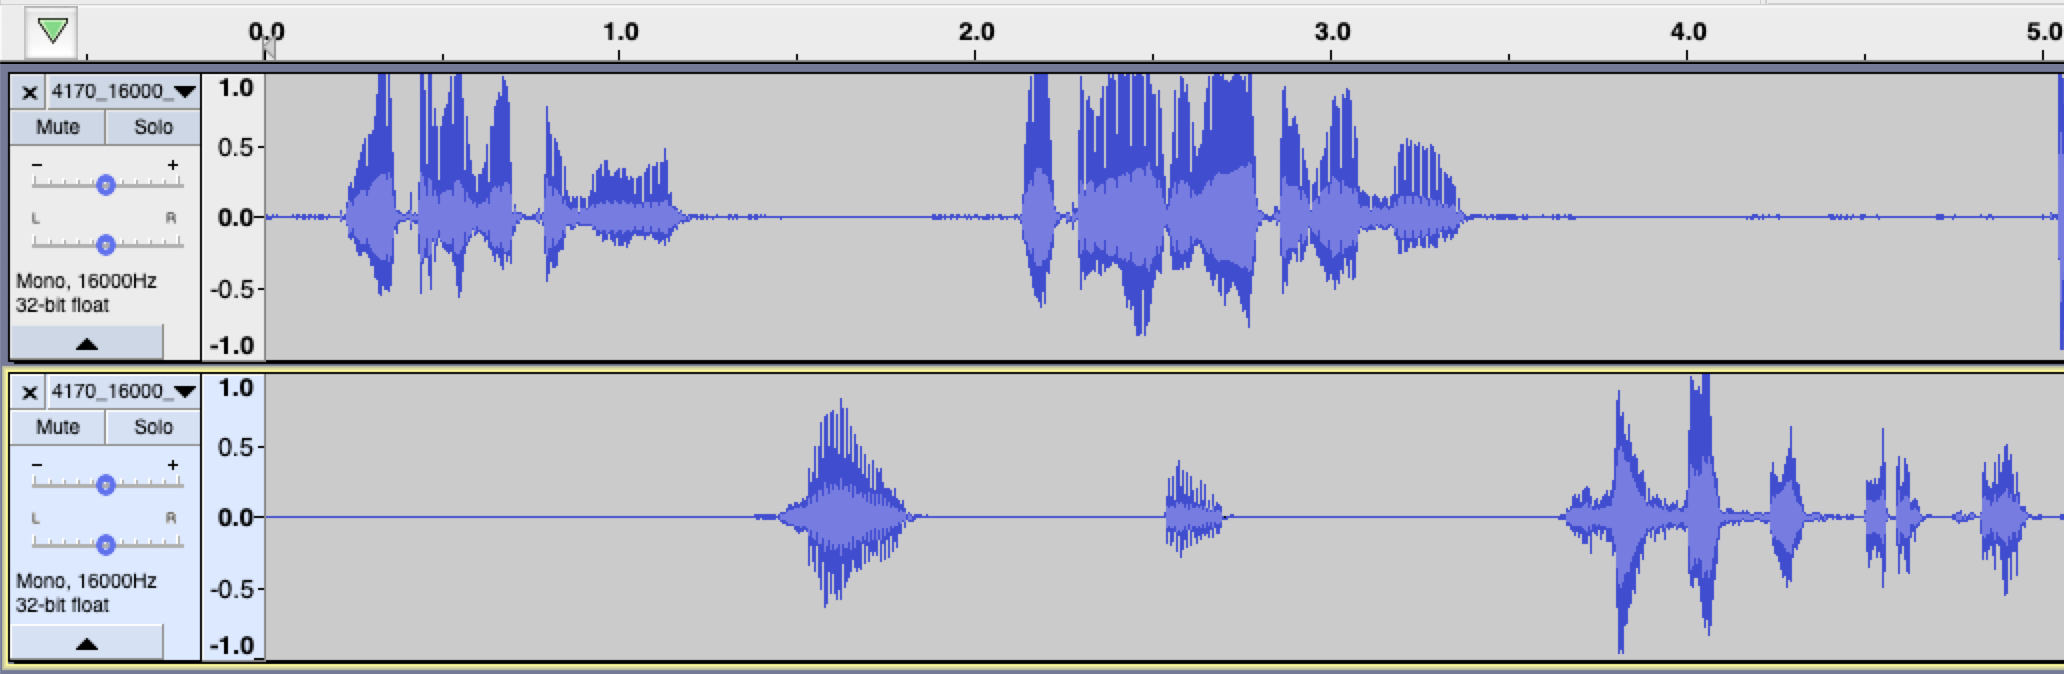
\includegraphics[scale=0.3]{src/main-matter/methodology/preliminary-testing/4170/waveform_4170_5s_chA_top_original}}
	\caption{44170 waveform - The first 5 seconds - Channel A top, Channel B bottom. Only sound present for Channel A, no sound present for Channel B.}
	\label{fig:upclose_sounding}
\end{figure}
\begin{figure}[h!]
	\centerline{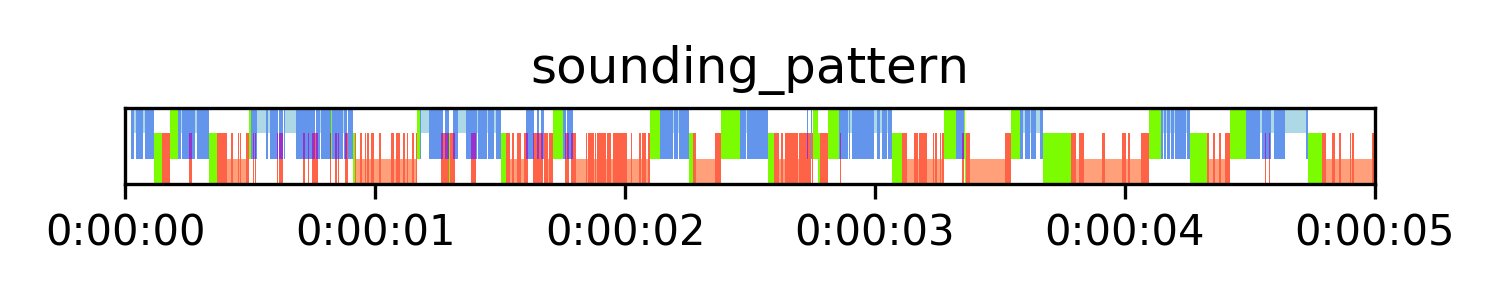
\includegraphics[scale=0.9]{src/main-matter/methodology/preliminary-testing/4170/sounding_pattern_plot_4170_mono_5s_range_short}}
	\caption{4170 Pause Code Plot - The first 5 seconds of audio - Channel A in blue - Channel B in red. Pause code shows more utterances for channel B than what exist in the waveform.}
	\label{fig:upclose_sounding}
\end{figure}



\subsection{Digitisation Process}
A wav file is read in using scipy.io.wavfile, this returns the sampling frequency of the audio file as well as a representation of the audio as an array. This is then sent to the dsp module where the pause and pitch profiles are created. From there the symbolisation process can occur.

\subsection{Digitisation Parameters}
\subsubsection{Time Step}
The Calpy.dsp module digitises the audio. The time\_step controls the level of granularity the audio files is digitised down to be. The smaller the number, the greater the resolution of the binary digitisation. The digitisation was done at the 100ms level, this was a good amount as digitisation returned high resolution results but took roughly 10-20 minutes to do (due to the long lengths of the audio), so decreasing the granularity down any further from the 100ms level would significantly hamper how much data can be retrieved (roughly an hour or two each file). 

\subsubsection{Minimum Silence}
Minimum audio silence is the minimum time required in an audio recording to mark that portion of audio as a silence. 1ms minimum silence was used. 

\subsubsection{Other parameters}
Frame\_window was an extra parameters that controlled the length of speech (in seconds) used to estimate pauses respectively. This was left as is at frame\_window = 0.025. 

\subsubsection{Pause Algorithm} 
This pause algorithm used in Calpy was taken from [Dynamical energy-based speech/silence detector for speech enhancement applications].
%[Sakhnov, K., Verteletskaya, E., \& Simak, B. (2009). Dynamical energy-based speech/silence detector for speech enhancement applications. Proceedings of the World Congress on Engineering (Vol. 1, p. 2).] \\
 

\newpage
\subsection{Pause Analysis}
%%%%%
% LANGUAGE - JAPAN v ENGLISH
%%%%%

%Although this isn't strictly good practice, combine together the groups that showed no difference intergroup on english and assume the same results would apply for Japanese. Once you get whole results for japanese and english then break down further. Just do this to try and get SOME kind of positive results at least. However, we may be bottlenecked by the pause code analysis and how many symbols we get back ultimately. 
%
%\paragraph{plots}
%Existing histograms (of interviews so not the same) and other graphs:
%A Large-Scale Multilingual Study of Silent Pause Duration by Estelle Campione \& Jean Véronis 
%The Duration of Speech Pauses in a Multilingual Environment by Mike Demol, Werner Verhelst, Piet Verhoeve 
%A Study of Speech Pauses for Multilingual Time-Scaling Applications by Mike Demol, Werner Verhelst, Piet Verhoeve 
%Different Interpretations of Pauses in Natural Conversation ---Japanese, Chinese and Americans by Yuka Shigemitsu*
%
%\paragraph{Work done so far}
%I've created a histogram of all the avg pauses of each audio file. 
%I've created a list of all outliers and done created histograms excluding anything below 200 (maybe 500?) (Should I exclude cases that are statistically out of the 60\% range?  Like below 300? above 1200? removing from below and above are signs that something went wrong in the test)
%So once outliers are removed I should show the before and after of the histogram?
%Histograms of the pause averages for all files, nothing below 200, and nothing below 400 show a clear tendency towards smaller pauses as the outliers are removed. This agrees with the results produced from the high quality abc interviews where the results showed the average pauses to be around xxx length. \\
%This test was used to try and find what pause numbers delivered the most consistent results to itself (so pauses not all over the place on a histogram) but also consistent with previous findings. As the low grade files were removed it became clear that more pauses tended to mean better quality output, but this wasn't always the case. Even some high output files, when examined closely, showed a tendency to over examine and assign pause (need to verify this if I'm going to say it). \\
%
%Which means fewer and fewer audio files that can be used to produce actual reliable results. The original number of files for jpn started at 119, the files that produced a total number of pauses above 200 was 55, and above 400 was 32. Although the database itself provides a large number of audio files, the vast majority are not reliable as a data source to draw decisive results from. Some files produced much higher values (~3500) indicating a need for further examination.These results are in contrast with the abc interview results where variance for those was xxxx, whereas variance for these are xxx. \\
%
%However, since work was already done to create the files, the results produced are given below. These may or may not provide some insight for future work. \\
%
%A best fit line was added to the histograms to help visualise what a normal dist might be over this sample set.
%  
%
%\paragraph{To Do:} 
%increase bin size for jpn_avgs, so many are around 100 that it becomes impossible to 

\newpage


\section{Model Success Evaluation}
The least complicated symbol model ended up being the best performing in terms of providing noticeable changes to the entropy profile. Simply by keeping the symbol model size down allowed for large changes in entropy to be easily noticeable. This was a significant result as it showed what was required for classification was actually just a very simple model, outperforming the more complicated SM[3,6,19,15]. \\

This allows for further complexity to be added if necessary but shows it's not inherently required. This model could be combined with other models that look at other pause types or even other prosodic speech elements to increase complexity. In those instances the symbol model approaches proposed allow for further investigation by considering alternate way to construct symbol models that might work better for other prosodic speech elements. Providing more options early on. 



\section{Symbol Model Comparisons}
\subsection{SA1}
Although SA1 is a very simple approach, SA1 worked very well as a classifier. The approach here was to utilise the fact that through the pause analysis investigation it was seen that shorter pauses were used more often by the older group while longer pauses were used by the younger group more often. \\

What was most interesting though was the effectiveness of a simple binary model regardless of obtaining the maximum entropy for a conversational group. As shown by SM[3] it was able to visualise the change in information content very well. It was shown to meet the constraints set out in the methodology required for an appropriate symbol model such as making sure every symbol is utilised, the symbol model size is appropriate for both the typical and atypical class, and it maximised the intergroup variance by making the two anomaly plots for young and middle aged as distinctly different as possible. The benefits are the simplistic approach to model building, it's very easy to see where the model is at its max and can be adjusted for easily by simply optimising the symbol split locations.\\

For SM[3] the margin was very minimal between the entropy profiles yet was able to accurately visualise the information content change. The reason this approach didn't work as well as SM[10] and SM[20] was it failing to take into account the change of both groups under this approach of maximum entropy, a byproduct of the model being that it raised the entropy profile significantly for the JJJ class as well. A better approach would be to focus on increasing the margin between the means by analysing the entropy profiles change in mean values as bin width is shifted and seeing how a model could be mathematically produced from this procedure automatically. \\

\subsection{Increasing Bin Width}
Interestingly the best performing models were SM[10] and SM[20] which increased the bin width of the simple binary model, these showed the significance symbol bin widths had on successful classification. This was due to the margin that existed between the means of the ABC and JJJ entropy profile for those models. The margins were much greater than they were for SM[3] meaning change was more noticeable. However SM[20] did employ the same principle as SM[3] which was to have one profile on the extreme of the information content value (ABC was at 0 entropy consistently) while the other was further away on the other end. \\ 


\subsection{SA2}
Adding complexity didn't necessarily make SM[3,6,10,15] any better in terms of obvious change in information content. An interesting result was how well it showed a change in entropy. The margin between SM[3] profiles was small yet showed a fairly noticeable dip in entropy, however SM[3,6,10,15] had an even greater change between the profile means yet showed very similar results to SM[3] in terms of noticeability of change. Further tests would look at the effect increasing symbol model size has on the resulting entropy profiles.\\
%
%SM[20] also showed it could successfully classify results however it suffered the same problem as SM[3] being it produced and entropy profile for typical that was too similar to the atypical group, thus making the distinction between the two profiles harder to see.\\ 
\subsection{Variance, Mean and Range Analysis}
Increasing symbol model size has completely opposite effects on the resulting mean and variance for the ABC and JJJ files when comparing SM[20] to SM[3,6,10.15]. It seemed no particular approach was able to control for variance and change in mean in the same manner consistently, however this is worth further investigation. Range and variance stayed roughly similar between JJJ for SM[10] and SM[20]. Knowing how to control for these parameters can lead to more effectively constructed models without requiring a 'guess and check' approach since the difference in information content is determined by how different the initial entropy profiles are.

\subsection{Audio Splicing Position}
Experiment 2.3 showed the change in entropy profiles when splicing position changed. SM[10] was shown to be invariant to this change meaning the significant results were not attributed to being in a special place in the conversation. This tells us change can be located anywhere in audio file as long as the proportion of change is high enough.

\subsection{SA3}
Although SA3 was never tested due to time constraints there was confidence in its approach to work that it would deliver effective results in further tests (by essentially doing what is being done now). This isn't to say that it would show all changes in entropy, as tests showed with the binary model it was not necessary for symbol model rankings reorder for change to be visualised. As shown in experiment 2.2.1, SM[10] produced the same symbol ranking for both ABC and JJJ files (ABC Ranked Probability: [(5294, 'A'), (138, 'B')], JJJ Ranked Probability: [(762, 'A'), (214, 'B')]). The significance here wasn't the change in symbol positioning but rather the change in proportions of those symbols.\\

This would work would due to symbol ranking reordering requiring large change in the proportion of symbol occurrence, thus by changing the order it would effectively be doing what we are looking for now. A benefit to this approach would be the robustness this model would have since a symbol model reordering is a distinct change that can be easily measured. However it is not seen how this is any different from setting a threshold of variance or mean change for the previous symbol models. \\

\subsection{Parameter Importance}
From the results it seemed that bin width played the most significant role in how the symbol model is constructed. However, limited experiment were run and only one higher complexity model was used (SM[3,6,10,15]). This could be investigated further to see the extent size has on entropy profile.

 
\section{Pause Classifier Evaluation}
Pauses have shown to be symbol model invariant, working with every symbol model proposed to give accurate change in information content. This means it has shown classification potential. Further tests would look into how reliable those results are by further testing this against other files and investigating the limits of the pause information content in age groups. \\

Next would look into how pauses are affected by language use and if age could be used alongside any significant results from that experiment to produce a model that utilises both aspects of a conversation to deliver even more accurate and reliable classification potential (e.g. looking at how age may affect pause use differently for speakers of different language). \\

\subsection{Cost}
The entire symbolisation approach is trivial to execute given the code written for it such that any one of the approaches outlined below could be run many times without cost as a way to explore the solution space. Experimenting with data here was aimed for given the almost zero cost in terms of time or energy here to run this process. \\

Given how easy these are to compute this means an online system wouldn't be strictly tied down to just one model. If the given model were to show an accurate classification on a small subgroup but high certainty, there's no reason more models like this couldn't be stacked together to create a more robust multi-model rather than a singular model that tries to handle all aspects of classification itself. \\

This would be beneficial for complex systems that require accurate classifications that have high amounts of computing power available (say industrial plants by analysing the information content from some procedure or machine in real time). This all depends on the type of system produced, some may require any change be reported and some may want classifications with a high degree of certainty. The take away being the ability to not be restricted to one model for use in an online system.\\



%\subsection{Further Tests}
%Increasing robustness by using the ranked symbol model to evaluate the margin between the symbols to try evaluating how to create  



%if the maximum entropy for a conversation or conversation group was found and significant change between groups was present. For Initial experiment 1 the entropy profile showed ...? . \\
%In the audio augmentation it proved to be better than the more complex model by separating the two groups into higher and lower entropy profiles much more clearly where both the mean and variance were adjusted thus making identification trivial. \\


%
%\subsubsection{Limitations}
%%It may also maximise entropy intergroup and thus you gain nothing but high entropy. 
%This method still requires a set threshold for change in entropy profile properties that signify an atypical data point has occurred, meaning extra parameters are still required for this (making it more complex). A downside of this approach could be a lack of moulding to the specific groups pause characteristics. Since the model is simply trying to maximise the entropy profile of the typical group this doesn't consider if this will be effective on the atypical group, offering no feedback on effectiveness as a classifier other than seeing if it works through experimentation. Ultimately this is much more of a heuristic approach to model building. This could mean the information disparity between groups being studied isn't being appropriately captured and potentially susceptible to intergroup variance not being accounted for, thus leading to poor classification results. \\
%
%\subsubsection{Benefits}
%The benefits are the simplistic approach to model building, it's very easy to see where the model is at its max and can be adjusted for easily by simply optimising the symbol split locations. This process can be automated by creating symbol models, computing the entropy profile, and the mean and variance of the profiles, then choosing the model that has the highest mean and lowest variance. This can potentially be solved for mathematically through gradient descent. 
%

%\subsection{SA2}
%The benefit of this approach is its simple to construct a model, similar to SA1. It's very similar in approach, the only difference being SA2 doesn't aim to maximise entropy. This was created incase potentially useful information is lost by maximising entropy for one group, however from the results shown this may not matter functionally. Although this was still able to produce 
%an identifier for locating atypical values in the entropy profile. 




%Symbolisation approach 2 was far less complicated by having less parameters and data sets to comb through. It was also easier to replicate from experiment to experiment which made results more consistent and faster, allowing for more iterations to be carried out if necessary.
%
%What about results?
%
%
%
%how many symbols\\
%symbol widths\\
%relationship between symbols (e.g. equiprobable bins)\\
%(from here we could increase the number of symbol sets so we can look at more data than just one type of pause, but thats waaaaay out of scope)\\
%desired distribution of symbols (do I want them to be equal in entropy or do i want them to follow the zml distribution? I think i want them to follow zml that way the fast entropy can use the zml its already modelled from?








%\newpage
% \subsubsection{Exp7 - [2, 3, 4, 5, 6, 7, 8, 9, 10]}

 \begin{table}[htp]
	\scriptsize
	\begin{center}
	\begin{tabular}
		{ 
			|p{1.5cm}| |p
			{1.5cm}|p
			{.8cm}|p
			{.8cm}|p
			{.8cm}|p
			{.8cm}|
		}
		\hline
		\multicolumn{6}{|c|}{ABC - Radio - Program: Conversations} \\%
		\hline
			{\footnotesize Audio File} & 
			{\scriptsize Entropy Variance} & 
			{\scriptsize Mode} &
			{\scriptsize Mean} &
			{\scriptsize Median} & 
			{\scriptsize Range} \\
		\hline
		\hline

		%\cellcolor[HTML]{A2A1A2} 
		aaj-2019-03-15 & 41 - 47 & 44 & - & - & 6 \\
		\hline 
		aaj-2019-03-21 & 40 - 48 & 44 & - & - & 8 \\
		\hline 
		aaj-2019-03-27 & 38 - 42 & 40 & - & - & 4 \\
		\hline
		aaj-2019-04-11 & 37 - 43 & 40 & - & - & 6 \\
		\hline
		aaj-2019-04-24 & 37 - 43 & 40 & - & - & 6\\
		\hline
		aaj-2019-04-26 & 41 - 48 & 44 & - & - & 7 \\
		\hline
		aaj-2019-04-29 & 38 - 46 & 42 & - & - & 8 \\
		\hline
		aaj-2019-04-30 & - & - & - & - & - \\
		\hline
		aaj-2019-05-17 & - & - & - & - & - \\
		\hline
		aaj-2019-05-08 & - & - & - & - & - \\
		\hline
		aaj-2019-05-09 & - & - & - & - & - \\
		\hline
		\hline 
		Average & - & - & - & - & 6.43 \\
		\hline
		\hline

	\end{tabular}
	\label{tab:1}
	\caption{Pause usage of abc conversations audio files - preliminary statistical pause analysis 
	pertaining to middle aged participants with the results of SM.1 on each audio file with the total pauses
	 for that file and the pauses counted for each symbol} \\
	\end{center}
\end{table}


 \begin{table}[htp]
	\scriptsize
	\begin{center}
	\begin{tabular}
		{ 
			|p{1.5cm}| |p
			{1.5cm}|p
			{.8cm}|p
			{.8cm}|p
			{.8cm}|p
			{.8cm}|
		}
		\hline
		\multicolumn{6}{|c|}{ABC - Radio - Program: Mornings} \\%
		\hline
			{\footnotesize Audio File} & 
			{\scriptsize Entropy Variance} & 
			{\scriptsize Mode} &
			{\scriptsize Mean} &
			{\scriptsize Median} & 
			{\scriptsize Range} \\
		\hline
		\hline

		%\cellcolor[HTML]{A2A1A2} 
		- & 38 - 42 & 40 & - & - & 4 \\
		\hline 
		-- & 37 - 41 & 39 & - & - & 4 \\
		\hline 
		--- & 37.5 - 41.5 & 39.5 & - & - & 4 \\
		\hline
		-- & 40 - 44 & 42 & - & - & 4 \\
		\hline
		-- & 37 - 42 & 39 & - & - & 5\\
		\hline
		--- & 38.5 - 41.5 & 40 & - & - & 3 \\
		\hline
		-- & 38 - 42 & 40 & - & - & 4 \\
		\hline
		---- & - & - & - & - & - \\
		\hline
		-- & - & - & - & - & - \\
		\hline
		-- & - & - & - & - & - \\
		\hline
		-- & - & - & - & - & - \\
		\hline
		\hline 
		Average & - & - & - & - & 4 \\
		\hline
		\hline

	\end{tabular}
	\label{tab:1}
	\caption{Pause usage of abc conversations audio files - preliminary statistical pause analysis 
	pertaining to middle aged participants with the results of SM.1 on each audio file with the total pauses
	 for that file and the pauses counted for each symbol} \\
	\end{center}
\end{table}




So what does high entropy mean, greater distributed use of the symbols? 

What does high variance mean then? Inconsistent use of pauses. Maybe it was the style of conversation? 

How is it higher variance? Are they hitting higher peaks? Lower troughs? 

What does it tell us about the groups? Maybe the longer length of conv allowed for different use of pauses (relaxed? does that account for the variance?)

This shows the variance tends to be greater for --- conversations, indicating the information theyre giving tends to move from high information to low more frequently whereas -- people tend to stick to a common entropy value more often.

Not only were the outlier points greater for conversations, but I think they tended to fluctuate more often between those points.





